% !TEX root = ./es-manual-main.tex


%% Based on a TeXnicCenter-Template by Gyorgy SZEIDL.
%%%%%%%%%%%%%%%%%%%%%%%%%%%%%%%%%%%%%%%%%%%%%%%%%%%%%%%%%%%%%

%------------------------------------------------------------
%
\documentclass{article}%
%Options -- Point size:  10pt (default), 11pt, 12pt
%        -- Paper size:  letterpaper (default), a4paper, a5paper, b5paper
%                        legalpaper, executivepaper
%        -- Orientation  (portrait is the default)
%                        landscape
%        -- Print size:  oneside (default), twoside
%        -- Quality      final(default), draft
%        -- Title page   notitlepage, titlepage(default)
%        -- Columns      onecolumn(default), twocolumn
%        -- Equation numbering (equation numbers on the right is the default)
%                        leqno
%        -- Displayed equations (centered is the default)
%                        fleqn (equations start at the same distance from the right side)
%        -- Open bibliography style (closed is the default)
%                        openbib
% For instance the command
%           \documentclass[a4paper,12pt,leqno]{article}
% ensures that the paper size is a4, the fonts are typeset at the size 12p
% and the equation numbers are on the left side
%
\usepackage{amsmath}%
\usepackage{amsfonts}%
\usepackage{amssymb}%
\usepackage{graphicx}
\usepackage{float}
\usepackage{pdfpages}

%\usepackage{amsmath}%
%\usepackage{amsfonts}%
%\usepackage{amssymb}%
%\usepackage{graphicx}
%\usepackage{subfigure}
\usepackage{subfig}

%\usepackage{amsmath}
\usepackage{amsthm}



% To construct algorithms.
%%% \usepackage[section]{algorithm} % [section] is use to define the numbering mode
%%% \usepackage{algorithmic} 

%%%
%%% Algorithms.  Don't have to use end for, etc.
\usepackage[ruled, vlined]{algorithm2e}


% For underlines.  The \normalem returns \emph to italics (not underline).
% To make wavy underline, use \uwave{boat} wavy underline
% see http://www.cvrti.utah.edu/~macleod/latex/
\usepackage{ulem}
\normalem

% For 'wingdings' (e.g., the right arrow, as in "as goes to infinity" -->OO.
\usepackage{pifont}

% For color text.
\usepackage{color}

% Long tables.
\usepackage{xtab}

\usepackage{multirow}

% For fields.
\newcommand{\field}[1]{\mathbb{#1}}


%% Horizontal lines in doc.
\newcommand{\HRule}{\rule{\linewidth}{0.5mm}}

% Font size
% 10 pt \small
% 12 pt \large
%\small


% Bibliography formatting.
% \usepackage{harvard}
% Reference styles,formats.
% See http://merkel.zoneo.net/Latex/natbib.php for details.
% The following is the manual:  http://www.ctex.org/documents/packages/bibref/natbib.pdf
%\usepackage{natbib}
%\bibpunct{(}{)}{;}{a}{,}{,}

% Path to figures.
\graphicspath{{./figures/}}

\newcommand{\figsize}{0.65}
\newcommand{\smallfigsize}{0.4}



% Code name and version.

\usepackage[top=1in, bottom=1in, left=1in, right=1in]{geometry}

%-------------------------------------------
\newtheorem{theorem}{Theorem}
\newtheorem{acknowledgement}[theorem]{Acknowledgement}
%\newtheorem{algorithm}[theorem]{Algorithm}
\newtheorem{axiom}[theorem]{Axiom}
\newtheorem{case}[theorem]{Case}
\newtheorem{claim}[theorem]{Claim}
\newtheorem{conclusion}[theorem]{Conclusion}
\newtheorem{condition}[theorem]{Condition}
\newtheorem{conjecture}[theorem]{Conjecture}
\newtheorem{corollary}[theorem]{Corollary}
\newtheorem{criterion}[theorem]{Criterion}
\newtheorem{definition}[theorem]{Definition}
\newtheorem{example}[theorem]{Example}
\newtheorem{exercise}[theorem]{Exercise}
\newtheorem{lemma}[theorem]{Lemma}
\newtheorem{notation}[theorem]{Notation}
\newtheorem{problem}[theorem]{Problem}
\newtheorem{proposition}[theorem]{Proposition}
\newtheorem{remark}[theorem]{Remark}
\newtheorem{solution}[theorem]{Solution}
\newtheorem{summary}[theorem]{Summary}
%\newenvironment{proof}[1][Proof]{\textbf{#1.} }{\ \rule{0.5em}{0.5em}}


%\newcommand{\hatnhl}{\mbox{$\mathcal{C}$}}
\newcommand{\hatnhl}{\hat{N}_{hl}}


\begin{document}


\title{MARS Network Services User Manual\\
Version 2.0}

\author{Sherif Abdelhamid, Chris Kuhlman}

\date{\today}
\maketitle


\tiny

\HRule \\[0.05cm]

\HRule \\[0.05cm]

\small

\tableofcontents

\tiny

\HRule \\[0.05cm]

\HRule \\[0.05cm]

\normalsize


% -------------------------------------------
\begin{abstract}

The purpose of this document is to provide an overview of MARS services, installation and usage.

\end{abstract}


% -------------------------------------------



% -------------------------------------------
\section{Introduction}


\subsection{What is MARS?}
MARS is a new network services and workflow system that supports structural network analyses and generalized network dynamics analyses. It is accessible through the internet and can serve multiple simultaneous users and software applications. In addition to managing various types of digital objects including networked data, MARS
provides services that enable applications (and UIs) to add, interrogate, query, analyze, and process data.

\begin{figure}[H]
\centering
%\label{fig:ebola-kshell-not-effective}
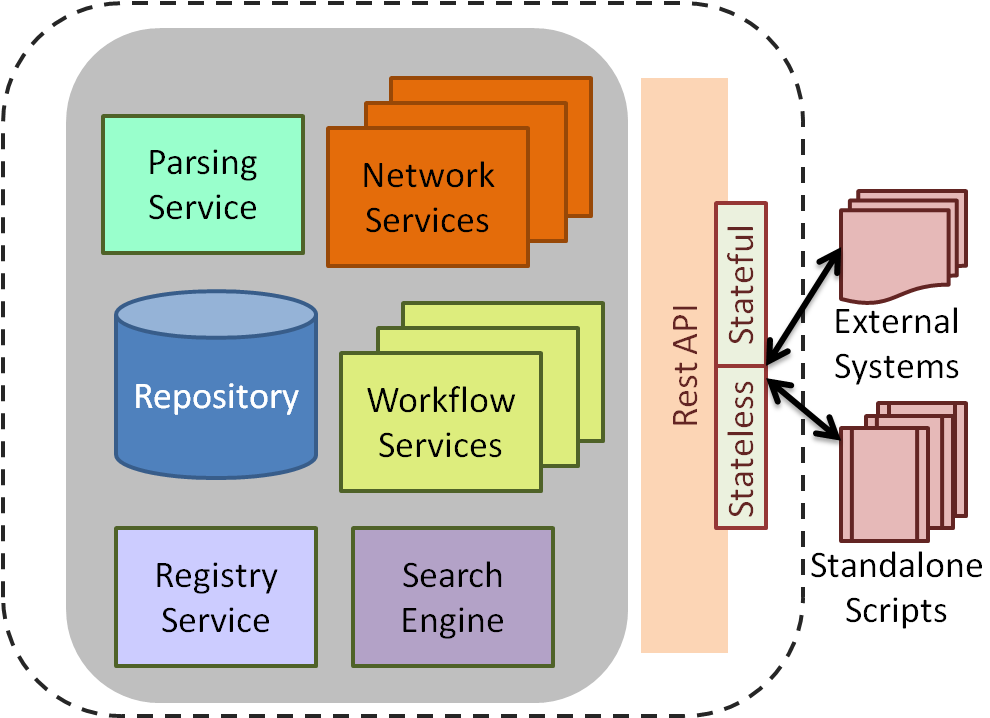
\includegraphics[trim = 0.0in 0.0in 0.0in 0.0in,scale=0.4]{mars-overall}
\caption{
Overview of the MARS system.
}   %   
\label{fig:mars-overall}
\end{figure}

\subsection{Features}

\begin{itemize}
\item Modular, interoperable categories
of services, where each service can be a distinct, relocatable process.
\item Stateless (REST-ful) and stateful (using session management) API.
\item SQL-like query grammar with special features for network dynamics.
\item Built-in search engine, for quey grouping, sharing and retrieval.
\item Database for storing networked data along with metadata.
\item \textbf{New in v2.0} Distributed architecture, multiple services run separately  on different VMs. Services communicate using HTTP requests.
\item \textbf{New in v2.0} Workflow service to execute a set of user-defined steps for analyzing networked data.
\item \textbf{New in v2.0} Data plotting service. Integrated within the workflow service. Currently, is using matplotlib but can be extended to other 3rd party plotting tools (e.g. ggplot, D3).
\item \textbf{New in v2.0} Network Measure service with a dedicated broker. The measure service has to be running on shadowfax.
\item \textbf{New in v2.0} Extended database schema.



\end{itemize}




\line(1,0){500}

\section{MARS Setup}

\subsection{Installation}


Currently, MARS v2.0 is tested to run on Linux platform. To install MARS:

\subsubsection{Python Installation}
\begin{itemize}
\item wget https://www.python.org/ftp/python/2.7.9/Python-2.7.9.tgz
\item tar -xzvf Python-2.7.9.tgz
\item cd Python-2.7.9
\item ./configure --prefix=[Python installation directory]
\item make
\item make test
\item make install

\end{itemize}


\subsubsection{Installing Required Packages}
\begin{itemize}
\item Check if pip or easy\_install are installed, if not do: 
\begin{itemize}
\item wget https://bootstrap.pypa.io/get-pip.py
\item python get-pip.py
\item wget https://bootstrap.pypa.io/ez\_setup.py $-$o $-$ $|$ python
\item easy\_install pip
\end{itemize}
\item Use pip or easy\_install to install the packages in Table~\ref{tab:modules} (e.g. easy\_install numpy or pip install whoosh):
\begin{table}[h]
\captionsetup{justification=justified,
singlelinecheck=true
}
\small{
\caption{List of python packages used for MARS implementation.
}

\begin{tabular}{|p{1.2in}| p{1.8in}| p{2.7in}|}
\hline 
\textbf{Package} & \textbf{Purpose}  &\textbf{Source}\\ 
\hline 
SQLITE & Data Repository & https://sqlite.org/\\
\hline 
Cherrypy & Multi-threaded python server & http://cherrypy.org/\\
\hline 
Whoosh & Search Engine & https://pypi.python.org/pypi/Whoosh/\\
\hline 
Pyparsing & Parser Generator & http://pyparsing.wikispaces.com/\\
\hline 
Bottle Framework & Rest API & http://bottlepy.org/docs/dev/\\
\hline 
MPipe & User-defined Workflows & http://vmlaker.github.io/mpipe/\\
\hline 
matplotlib  & Data Plotting & http://matplotlib.org/\\
\hline 
pythonds & Internal Data Structures (Stack) & https://pypi.python.org/pypi/pythonds\\
\hline 
requests & Send/Receive HTTP Requests & http://docs.python-requests.org/en/master/\\
\hline 
NumPy & Data Analysis & http://www.numpy.org/\\
\hline
NetworkX & Network Structure Measures & https://networkx.github.io/\\
\hline
\end{tabular}
\label{tab:modules}
}
\end{table}
\end{itemize}	

\subsubsection{Creating a mounted directory}
\begin{itemize}
\item Currently, there is a mounted directory on shadowfax "/home/sipcinet/edison/graphservices" that is shared with edisondev VM. The same directory is accessed from edison VM at "/home/sip/edison/graphservices". The directory is needed for sharing files and codes between the measure service which is running on shadowfax and the rest of services running on other VMs. This setting relieve the services from handling large file transfers and share the same configuration setup (mars.config).
\item To create a new mounted directory between shadowfax and a new VM, please contact the RT at VBI. Go to rt.vbi.vt.edu and create a new ticket.
\end{itemize}

\subsubsection{Downloading MARS Code}
Note: it is preferred to download the mars v2.0 code to any place within the mounted directory. This provides flexibility in starting and stopping the services.
\begin{itemize}
\item Ask Sherif Abdelhamid (sherief@vbi.vt.edu) or Chris Kuhlman(ckuhlman@vbi.vt.edu) to be added to git project (https://ndsslgit.vbi.vt.edu/software-contagion-services/network-services)
\item enter git clone https://ndsslgit.vbi.vt.edu/software-contagion-services/network-services.git
\item cd network-services
\item check the main directories v1 and v2. Each directory has two sub-directories src (code) and doc (manual).
\item v2.0 codes resides under v2/src sub-directory.
\item Copy database file into a database directory of your choice (This is a database directory that you created or have access permission to it. Please make sure that it doesn't contain a database file with the same name. It is preferable to use a sub-directory under the mounted directory). \\
scp username@edisondev.vbi.vt.edu:/home/sipcinet/edison/graphservices/database/Edison2.db [database directory]
\end{itemize}

\subsubsection{configuring MARS services}
\begin{itemize}
\item go to [code directory]/v2/src/code
\item check and edit (if needed) the properties:
\begin{itemize}
\item server: name of the python server used. Currently, set to cherrypy, a multithreaded server written python.
\item host: server IP address that will host MARS. It can be set to localhost. 
\item port: list of port numbers that will be used. Each port number is in a separate line. Two services can not share the same port. Make sure when add port to the config file that only one service can use at a time.
\item database: the database directory.
\item index1: location where property queries are indexed on the file system.
\item index2: location where seed queries are indexed on the file system.
\item query: directory where query results are stored on the file system.
\item workflow: \textbf{New in v2.0} location where the plots generated by workflow services are stored. [need to be under the NEMO webapp directory]
\item uploadfile: \textbf{New in v2.0} directory where uploaded files by NEMO web-interface are stored. [need to be under the NEMO webapp directory]
\item qsub and output: \textbf{New in v2.0} two directories used by the measure service in MARS v2. Store information about qsub execution for network measures.
\item graph: directory for MARS graphs.
\item code: the directory that contains the services code and the stand-alone executable codes that compute measures on networks.  These codes can be C, C++, Python, Perl, or codes written in any other language.  These are called by the measure service in MARS v2.0. 
\item notify\_storage: \textbf{New in v2.0} A flag (True/False) to determine whether the measure service will notify the network storage service to store the computed measure or not. If you choose False then you can add the network manually, see Section~4 for more details.

\end{itemize}
\end{itemize}


\subsubsection{Starting Network Measure Service on shadowfax}
Note: the measure service has to run on shadowfax to be able to submit a job using qsub. Shadowfax has a cluster management server running on the headnode (sfx1, sfx2, ..). This server monitors the status of the cluster and controls/monitors the various queues and job lists. qsub interacts with the server and lets it know that there is another job that has requested resources on the cluster. Other services can run on other VMs or shadowfax.
\begin{itemize}
\item sudo su - sipcinet
\item export PATH=[python installation directory on shadowfax]:\$PATH
\item go to [code directory]/v2/src/code 
\item to start the measure service enter python measure\_service2.py \&
\item to start the measure broker used by the measure service (monitor the job submission status) enter measure\_broker \&.
Note: the measure service is now running on shadowfax.
 
\end{itemize}


\subsubsection{Starting MARS Services on edisondev}
Note: the same steps can be done on other VMs, as long as the user has the required permissions and access rights. Since multiple services can run on the same machine, please make sure to assign different port for each service. 
\begin{itemize}
\item sudo su - sipcinet
\item export PATH=[python installation directory]:\$PATH
\item go to [code directory]/v2/src/code
\item to start the query service enter python query\_service2.py \&
\item to start the storage service enter python storage\_service2.py \&
\item to start the workflow service enter python workflow\_service2.py \&
Note: the storage, workflow, and query services are now started on edisondev. Each service has its own port that is defined in mars.config file.
\end{itemize}







\subsubsection{Stopping MARS Services}
Note: this steps can repeated for each process/service. A shell script can be written to speed up the task.
\begin{itemize}
\item ps ax $|$ grep python [Retrieve python process PID]
\item kill $-$9 PID

\end{itemize}

\subsubsection{Create index for Network Query Search Service}

\begin{itemize}
\item go to [code directory]/v1/src/code
\item enter python create\_index.py [This will create two indexes, for the property and seed type queries]. The indexes directories are specified in the mars.config file as index1 and index2.
\end{itemize}
note: after creating the indexes make sure to give read/write permissions to all the files under index1 and index2. Use this command chmod 666 *.*




\subsection{Contribution steps}
To start contributing to MARS repository, please follow these steps:
\begin{itemize}
\item Create a new branch and switch to it [git checkout $-$b [name\_of\_your\_new\_branch]. Name of branch should begin with class type:
\begin{itemize}
\item Feature, if user is adding a new feature for MARS.
\item Bug-fix, if user updating current code to fix a bug.
\item Enhancement, if user is updating current code for code optimization or performance enhancement.
\end{itemize} 

\item Commit the changes with a  descriptive message. [git commit -m "Commit message"]. 
\item Create a new remote for your branch [git remote add [name\_of\_your\_remote]].
\item Push the branch to the remote repository [git push [name\_of\_your\_new\_remote] [name\_of\_your\_new\_branch]].
\item Create a merge request using https://ndsslgit.vbi.vt.edu, as shown in Figure~\ref{fig:merge-request}. Notify other team members to review.
\item Reviewer will check for merge conflicts.
\item Reviewer merge the new branch with master.

\begin{figure}[H]
\centering
%\label{fig:ebola-kshell-not-effective}
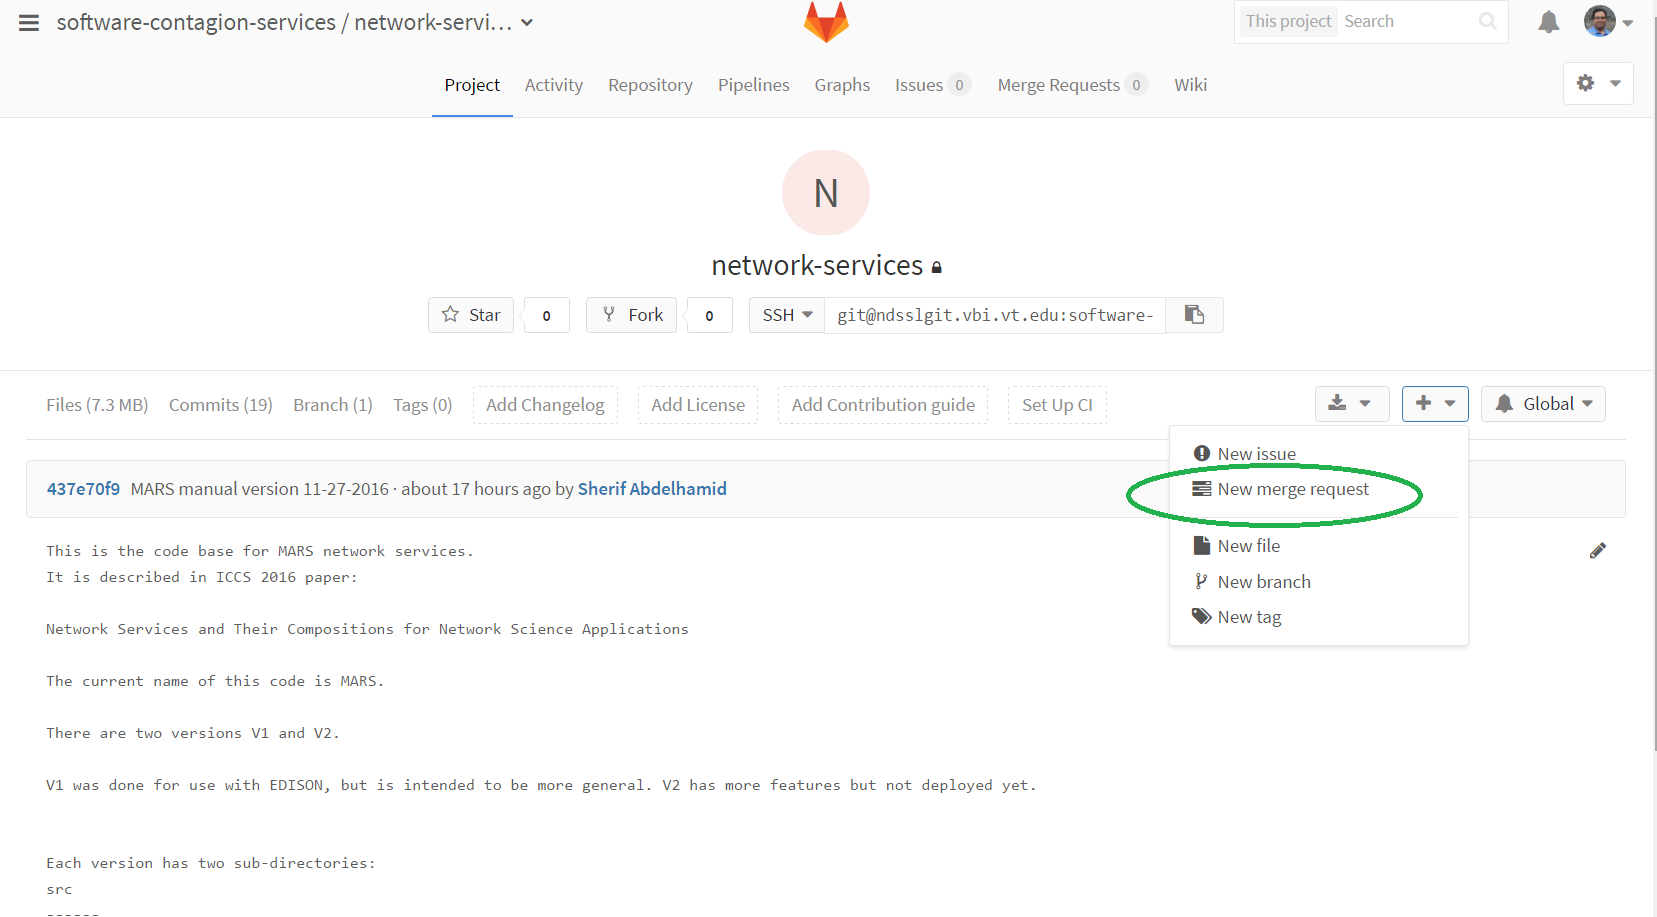
\includegraphics[trim = 0.0in 0.0in 0.0in 0.0in,scale=0.55]{merge-request}
\caption{
Creating a merge request using Web-based interface of ndsslgit.
}   %   
\label{fig:merge-request}
\end{figure}

\end{itemize}





\line(1,0){500}

\input{Using-MARS}

\line(1,0){500}
\section{Adding New Networks Manually}
MARS v2.0 has the capability to add networks automatically. However, users can still manually add networks as in v1.0. Manual approach can be useful with large networks.
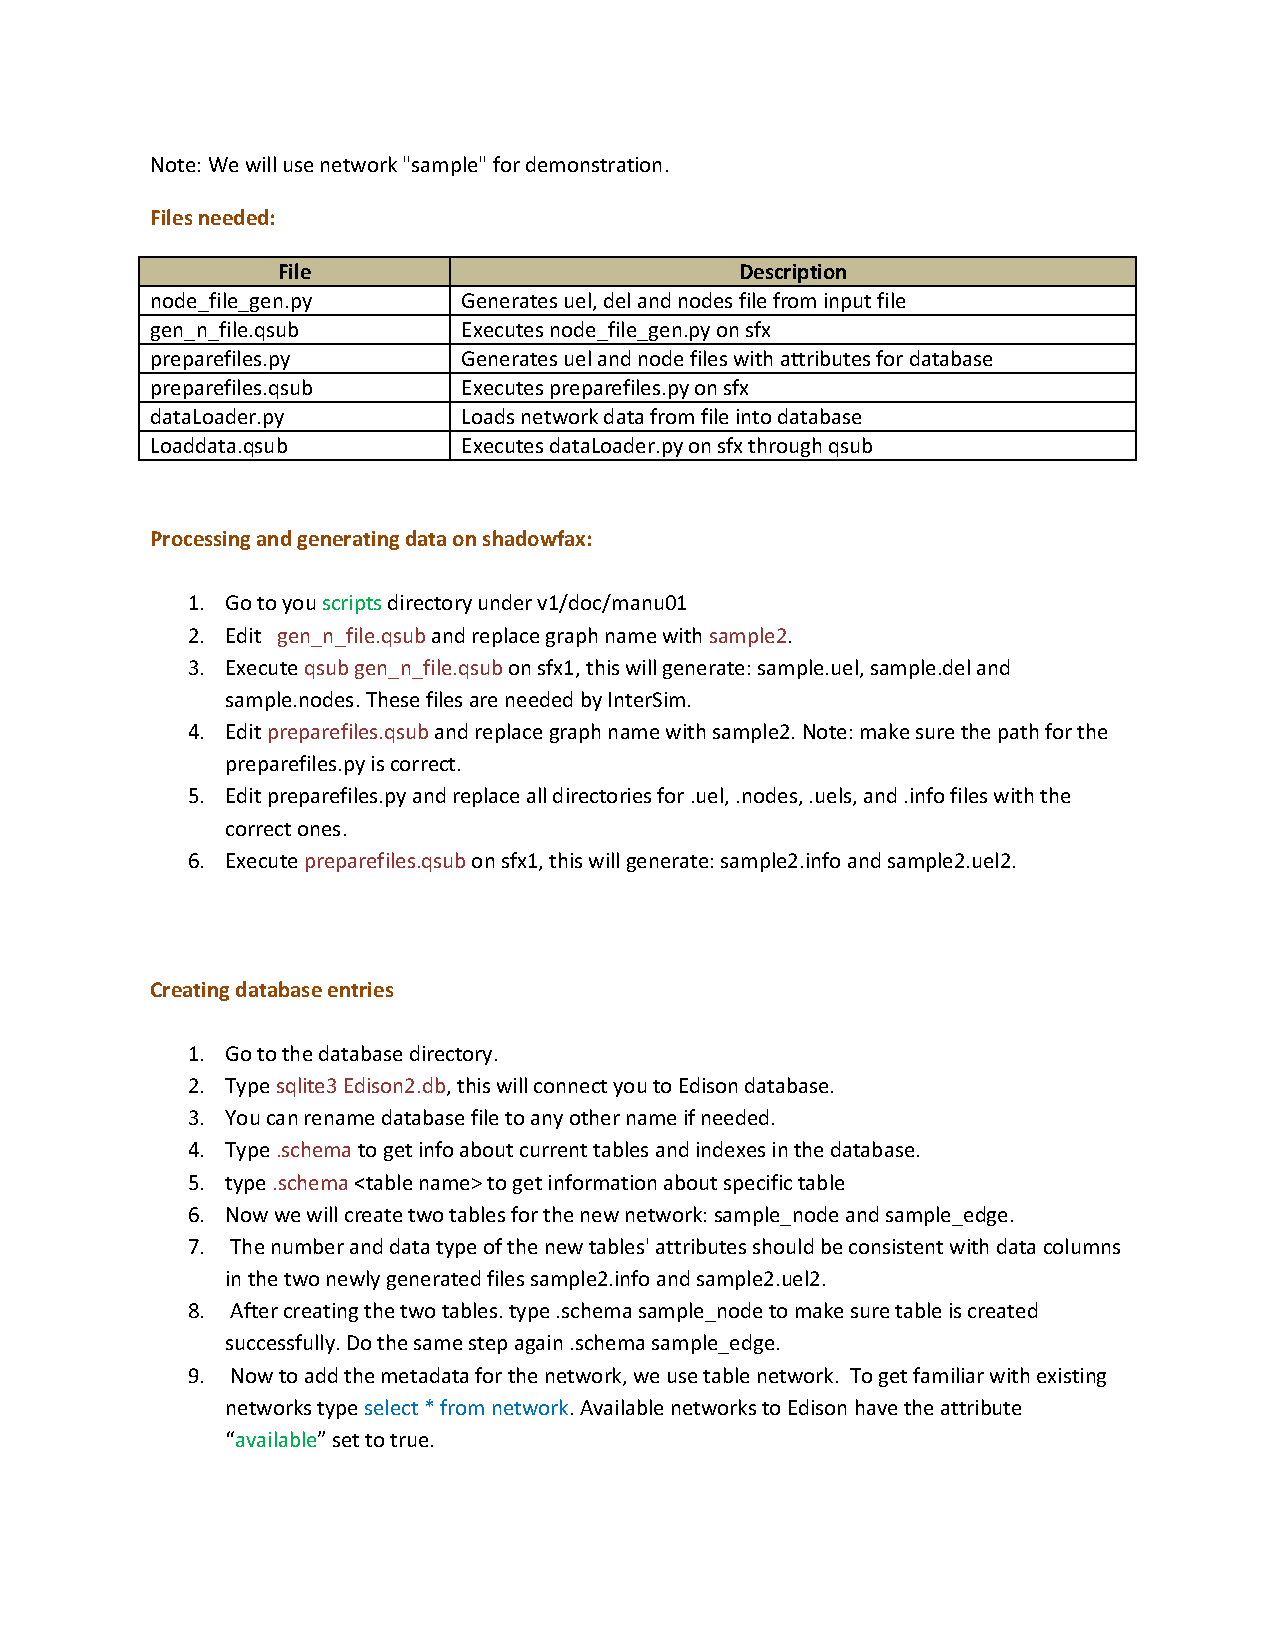
\includepdf[pages={-}]{add-networks.pdf}


\line(1,0){500}
% -------------------------------------------
\section{Verification Testing}
Note: verification testing are used to validate MARS services output after every code change (e.g. new feature). A set of python scripts were prepared to automate the tests. There are three separate directories under the [code directory]/v2/src/code/verification directory that contain the python scripts and the valid output files (with extension .valid). Some of the verification scripts don't use .valid files, the data is hard-coded in the python script file.

\begin{itemize}
\item go to [code directory]/v2/src/code/verification. 
\item to verify the measure service go to dir /measure\_service and enter measure\_verify.py. Note: the measure service should runs on shadowfax. 
\item to verify the query service go to dir /query\_service and enter query\_verify.py. 
\item to verify the workflow service go to dir /workflow\_service and enter workflow\_verify.py.


\end{itemize}
Note: the ordering of testing the services should be consistent with the above ordering. The sample and sample2 networks are used for the verification testing. Please run reset\_sample.py, found at directory [code directory]/v2/src/code/verification, before starting the tests. This will reset the database state and remove any priori computations for these two networks.

%
% ---- Bibliography ----
%

%\bibliographystyle{plain}
%\bibliography{refs-mnf-files}




\end{document}
